%%%%%%%%%%%%%%%%%%%%%%%%%%%%%%%%%%%%%%%%%%%%%%%%%%%%%%%%%%%%%%%
%
%
%%%%%%%%%%%%%%%%%%%%%%%%%%%%%%%%%%%%%%%%%%%%%%%%%%%%%%%%%%%%%%%

\documentclass{article}
\usepackage{graphicx}
\usepackage{fullpage}
\usepackage{amsmath}

\title{Übungsblatt 5}
\author{Tobias Baake (247074), Dylan Ellinger (247316), Nikiforos Tompoulidis (247714)}
\begin{document}
\maketitle

\section{Delaunay-Triangulierung}


\section{Dreiecksqualität}
\emph{a)}\\
\\
Eckpunkte:
\\\\
( A(0, 1, 0) ), ( B(0, 0, 1) ), und ( C(1, 0, 0) ).
\\\\
Seitenlängen:
\\
$ d = \sqrt{(x_2-x_1)^2 + (y_2-y_1)^2 + (z_2-z_1)^2} $
\\\\
Die Seitenlängen des Dreiecks ABC sind dann:
\\
( a = |BC| ), ( b = |AC| ), und ( c = |AB| ).
\\\\
Berechnung:
\\
$ a = \sqrt{(1-0)^2 + (0-0)^2 + (0-1)^2} = \sqrt{1+0+1} = \sqrt{2} $
\\
$ b = \sqrt{(1-0)^2 + (0-1)^2 + (0-0)^2} = \sqrt{1+1+0} = \sqrt{2} $
\\
$ c = \sqrt{(0-0)^2 + (1-0)^2 + (0-1)^2} = \sqrt{0+1+1} = \sqrt{2} $
\\
\\
Da alle Seiten gleich lang sind (es handelt sich um ein gleichseitiges Dreieck), ist jede Seite die kürzeste Kantenlänge, also ist $ \min{a, b, c} = \sqrt{2} $.
\\
Der Halbumfang ( p ) des Dreiecks ist:
\\
$ p = \frac{a + b + c}{2} = \frac{\sqrt{2} + \sqrt{2} + \sqrt{2}}{2} = \frac{3\sqrt{2}}{2} $
\\\\
Nun können wir den Radius ( r ) des Umkreises mithilfe der gegebenen Formel berechnen:
\\
$ r = \frac{abc}{\sqrt{(a + b + c)(b + c - a)(c + a - b)(a + b - c)}} $
\\
Mit $ a = b = c = \sqrt{2} $, erhalten wir:
\\
$ r = \frac{(\sqrt{2})(\sqrt{2})(\sqrt{2})}{\sqrt{(3\sqrt{2})(\sqrt{2})(\sqrt{2})(\sqrt{2})}} = \frac{2\sqrt{2}}{\sqrt{6\sqrt{2}}} = \frac{2\sqrt{2}}{\sqrt{2}\sqrt[4]{6}} = \frac{2}{\sqrt[4]{6}} $
\\\\
Schließlich ist die Qualität ( q ) des Dreiecks:
\\
$ q = \frac{r}{\text{kürzeste Kantenlänge}} = \frac{2/\sqrt[4]{6}}{\sqrt{2}} = \frac{2}{\sqrt{2} \cdot \sqrt[4]{6}} = \underline{\underline{\frac{\sqrt{2}}{\sqrt[4]{6}}}} $
\\\\
\emph{b)}\\
Eckpunkte:
\\
$ A(2, 1),$ $B(\frac{5}{2}, 2)$, und $C(0, 3) $
\\\\
Seitenlängen:
\\
$ a = \sqrt{(\frac{5}{2}-0)^2 + (2-3)^2} = \sqrt{\frac{25}{4} + 1} = \sqrt{\frac{29}{4}} = \frac{\sqrt{29}}{2} $
\\
$ b = \sqrt{(2-\frac{5}{2})^2 + (1-2)^2} = \sqrt{\frac{1}{4} + 1} = \sqrt{\frac{5}{4}} = \frac{\sqrt{5}}{2} $
\\
$ c = \sqrt{(0-2)^2 + (3-1)^2} = \sqrt{4 + 4} = \sqrt{8} = 2\sqrt{2} $
\\
Die kürzeste Kantenlänge des Dreiecks ist $ \min{a, b, c} = \frac{\sqrt{5}}{2} $.
\\\\
Halbumfang $ p $:\\
$ p = \frac{a + b + c}{2} = \frac{\frac{\sqrt{29}}{2} + \frac{\sqrt{5}}{2} + 2\sqrt{2}}{2} $\\
$ p = \frac{\sqrt{29} + \sqrt{5} + 4\sqrt{2}}{4} $
\\\\
% Using area formula and circumradius formula to find r without mentioning the semiperimeter explicitly
Der Umkreisradius \( r \) eines Dreiecks mit den Seitenlängen \( a \), \( b \), und \( c \) ist gegeben durch:\\
$ r = \frac{abc}{4A} $\\
wo \( A \) der Flächeninhalt des Dreiecks ist:\\
$ A = \sqrt{p(p - a)(p - b)(p - c)} $\\
Hierbei ist \( p \) der Halbumfang des Dreiecks.\\
\\
Kombiniert ergibt sich für \( r \):\\
$ r = \frac{abc}{4\sqrt{p(p - a)(p - b)(p - c)}} $
\\\\
Schließlich ist die Qualität \( q \) des Dreiecks:\\
$ p = \frac{\sqrt{29} + \sqrt{5} + 4\sqrt{2}}{4} $\\
$ q = \frac{\sqrt{290}}{2\sqrt{5}} \cdot \frac{1}{\sqrt{16p(p - a)(p - b)(p - c)}} $\\
$ q = \frac{\sqrt{290}}{2\sqrt{5}} \cdot \frac{1}{\sqrt{16 \left( \frac{\sqrt{29} + \sqrt{5} + 4\sqrt{2}}{4} \right) \left( \frac{\sqrt{29} + \sqrt{5} + 4\sqrt{2}}{4} - \frac{\sqrt{29}}{2} \right) \left( \frac{\sqrt{29} + \sqrt{5} + 4\sqrt{2}}{4} - \frac{\sqrt{5}}{2} \right) \left( \frac{\sqrt{29} + \sqrt{5} + 4\sqrt{2}}{4} - 2\sqrt{2} \right) }} $\\
\\\\
\section{Marching Viereck}
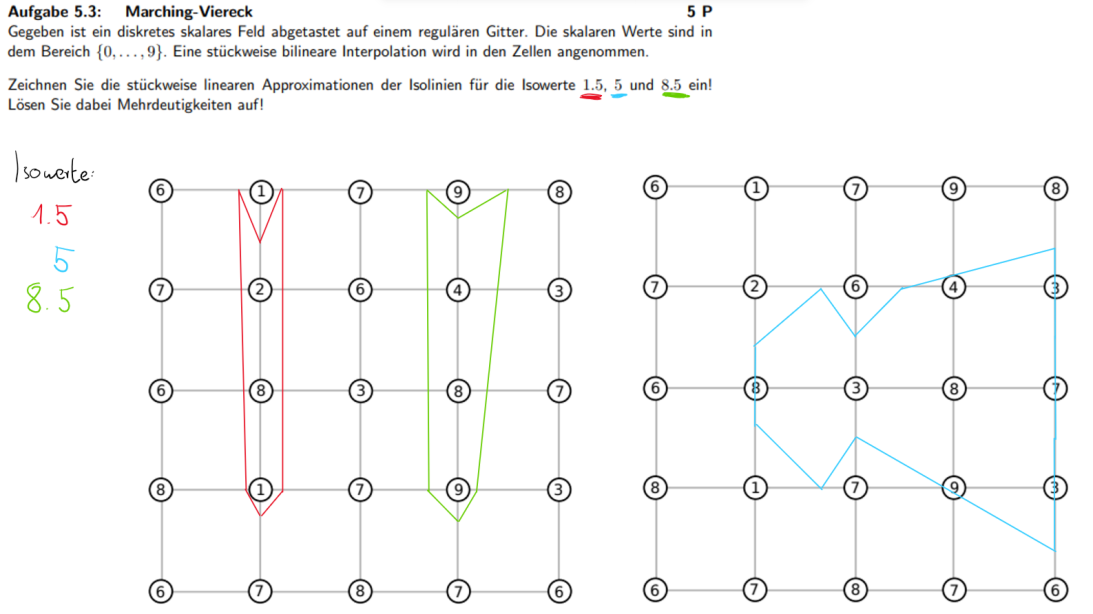
\includegraphics[width=400pt]{./files/Übung5.3.png}

\section{Marching Cubes}
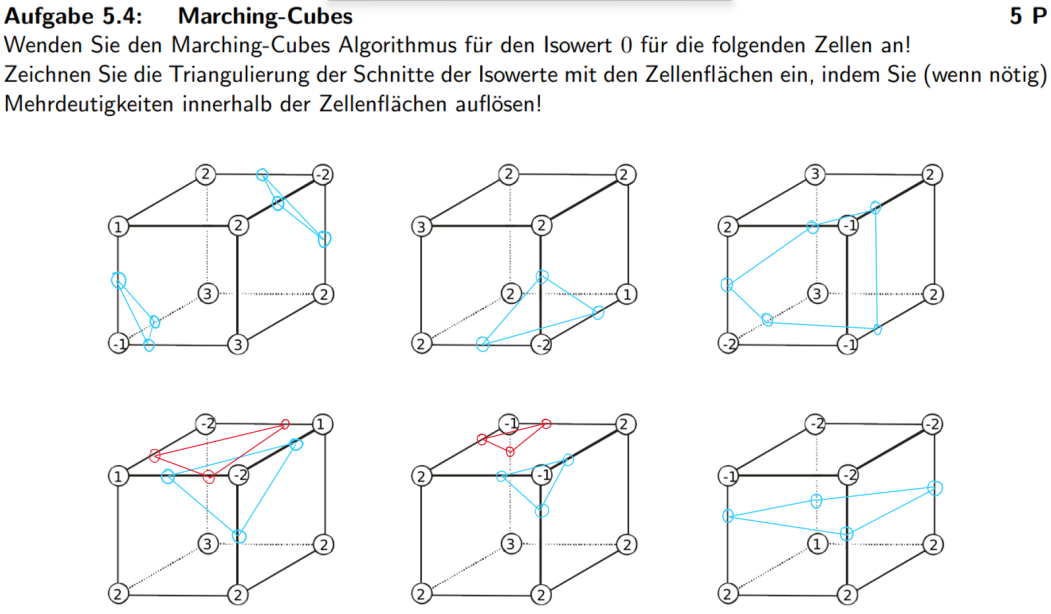
\includegraphics[width=400pt]{./files/Übung5.4.png}
\\
\\
\end{document}

